% ============================================================================
% INDUSTRY FOCUS ENHANCEMENTS
% ============================================================================
% This file contains enhancement slides for practical industry applications:
% 1. MLOps and Model Deployment
% 2. Data Quality and Monitoring
% 3. Business Stakeholder Communication
% 4. Regulatory Compliance and Ethics
%
% Author: Diogo Ribeiro
% Last Updated: January 5, 2025
%
% Integration: Include this file in your main presentation with \input{}
% or copy sections as needed. See INDUSTRY_FOCUS_ENHANCEMENT_GUIDE.md
% ============================================================================

% ============================================================================
% SECTION 1: MLOPS AND MODEL DEPLOYMENT
% ============================================================================

\section{MLOps and Model Deployment}

\begin{frame}{From Notebook to Production: The MLOps Challenge}
\begin{columns}
\begin{column}{0.5\textwidth}
\textbf{The Reality Gap:}
\begin{itemize}
\item 87\% of data science projects never make it to production \cite{venturebeat2019}
\item Average time to deploy: 8-12 months
\item 50\% of deployed models fail in first year
\end{itemize}

\vspace{0.3cm}
\textbf{Why Models Fail:}
\begin{enumerate}
\item Data drift and distribution shift
\item Integration complexity
\item Performance degradation
\item Inadequate monitoring
\item Technical debt accumulation
\end{enumerate}
\end{column}

\begin{column}{0.45\textwidth}
\begin{center}
\includegraphics[width=\textwidth]{figures/mlops_lifecycle.png}
\end{center}

\vspace{0.2cm}
\textbf{MLOps bridges the gap between:}
\begin{itemize}
\item \textcolor{navyblue}{ML development} (data scientists)
\item \textcolor{crimson}{Operations} (engineers)
\item \textcolor{forest}{Business} (stakeholders)
\end{itemize}
\end{column}
\end{columns}
\end{frame}

\begin{frame}{The MLOps Maturity Model}
\begin{table}
\centering
\small
\begin{tabular}{p{1.8cm}p{2.5cm}p{3cm}p{3.5cm}}
\toprule
\textbf{Level} & \textbf{Deployment} & \textbf{Training} & \textbf{Characteristics} \\
\midrule
\textcolor{crimson}{Level 0} & Manual & Manual & Notebooks, ad-hoc scripts \\
\midrule
\textcolor{gold}{Level 1} & Automated & Manual & CI/CD pipeline, version control \\
\midrule
\textcolor{forest}{Level 2} & Automated & Automated & Auto-retraining, feature store \\
\midrule
\textcolor{navyblue}{Level 3} & Automated & Automated & Full automation, real-time monitoring \\
\bottomrule
\end{tabular}
\end{table}

\vspace{0.3cm}
\textbf{Key Components at Each Level:}
\begin{itemize}
\item \textbf{Level 0 → 1:} Version control (Git), containerization (Docker), basic CI/CD
\item \textbf{Level 1 → 2:} Feature store, model registry, automated testing, monitoring
\item \textbf{Level 2 → 3:} Auto-retraining pipelines, A/B testing, real-time serving
\end{itemize}

\vspace{0.2cm}
\small\textit{Source: Google's MLOps Maturity Model \cite{google2021mlops}}
\end{frame}

\begin{frame}[fragile]{MLOps Architecture: Key Components}
\begin{center}
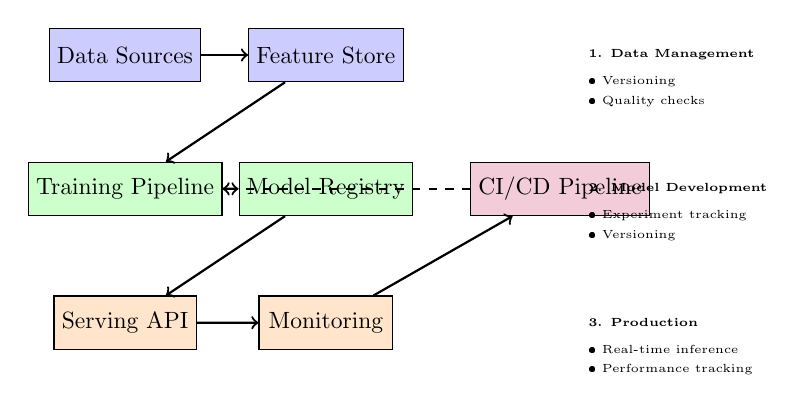
\begin{tikzpicture}[scale=0.85, every node/.style={scale=0.85}]
% Data layer
\node[draw, rectangle, fill=blue!20, minimum width=2cm, minimum height=0.8cm] (data) at (0,0) {Data Sources};
\node[draw, rectangle, fill=blue!20, minimum width=2cm, minimum height=0.8cm] (feature) at (3,0) {Feature Store};

% Training layer
\node[draw, rectangle, fill=green!20, minimum width=2cm, minimum height=0.8cm] (train) at (0,-2) {Training Pipeline};
\node[draw, rectangle, fill=green!20, minimum width=2cm, minimum height=0.8cm] (registry) at (3,-2) {Model Registry};

% Serving layer
\node[draw, rectangle, fill=orange!20, minimum width=2cm, minimum height=0.8cm] (serve) at (0,-4) {Serving API};
\node[draw, rectangle, fill=orange!20, minimum width=2cm, minimum height=0.8cm] (monitor) at (3,-4) {Monitoring};

% CI/CD
\node[draw, rectangle, fill=purple!20, minimum width=2.5cm, minimum height=0.8cm] (cicd) at (6.5,-2) {CI/CD Pipeline};

% Connections
\draw[->, thick] (data) -- (feature);
\draw[->, thick] (feature) -- (train);
\draw[->, thick] (train) -- (registry);
\draw[->, thick] (registry) -- (serve);
\draw[->, thick] (serve) -- (monitor);
\draw[->, thick] (monitor) -- (cicd);
\draw[->, thick, dashed] (cicd) -- (train);

% Labels
\node[anchor=west, font=\tiny] at (6.8,0) {\textbf{1. Data Management}};
\node[anchor=west, font=\tiny] at (6.8,-0.4) {• Versioning};
\node[anchor=west, font=\tiny] at (6.8,-0.7) {• Quality checks};

\node[anchor=west, font=\tiny] at (6.8,-2) {\textbf{2. Model Development}};
\node[anchor=west, font=\tiny] at (6.8,-2.4) {• Experiment tracking};
\node[anchor=west, font=\tiny] at (6.8,-2.7) {• Versioning};

\node[anchor=west, font=\tiny] at (6.8,-4) {\textbf{3. Production}};
\node[anchor=west, font=\tiny] at (6.8,-4.4) {• Real-time inference};
\node[anchor=west, font=\tiny] at (6.8,-4.7) {• Performance tracking};
\end{tikzpicture}
\end{center}

\vspace{0.2cm}
\textbf{Critical Integration Points:}
\begin{itemize}
\item Feature engineering consistency (training vs. serving)
\item Model versioning and rollback strategies
\item Automated testing and validation
\end{itemize}
\end{frame}

\begin{frame}[fragile]{Model Deployment Patterns}
\textbf{1. Batch Prediction (Offline Serving)}
\begin{lstlisting}[basicstyle=\ttfamily\tiny]
# Daily batch scoring job
import pandas as pd
from joblib import load

# Load model and data
model = load('model_v1.2.pkl')
data = pd.read_sql("SELECT * FROM customers WHERE score_date IS NULL", conn)

# Score in batches
predictions = model.predict(data[feature_cols])
results = pd.DataFrame({
    'customer_id': data['customer_id'],
    'churn_probability': predictions,
    'score_date': pd.Timestamp.now()
})

# Write to database
results.to_sql('churn_scores', conn, if_exists='append')
\end{lstlisting}

\textbf{Use cases:} Marketing campaigns, periodic reporting, risk assessment
\end{frame}

\begin{frame}[fragile]{Model Deployment Patterns (cont.)}
\textbf{2. Real-Time API (Online Serving)}
\begin{lstlisting}[basicstyle=\ttfamily\tiny]
from fastapi import FastAPI
from pydantic import BaseModel
import mlflow.pyfunc

app = FastAPI()
model = mlflow.pyfunc.load_model("models:/fraud_detection/production")

class Transaction(BaseModel):
    amount: float
    merchant_category: str
    hour_of_day: int
    days_since_last_transaction: float

@app.post("/predict")
async def predict_fraud(transaction: Transaction):
    # Feature engineering (must match training!)
    features = prepare_features(transaction)

    # Predict with latency monitoring
    start_time = time.time()
    prediction = model.predict(features)
    latency = time.time() - start_time

    # Log to monitoring system
    log_prediction(transaction, prediction, latency)

    return {
        "fraud_probability": float(prediction[0]),
        "latency_ms": latency * 1000,
        "model_version": model.metadata.version
    }
\end{lstlisting}

\textbf{SLA Requirements:} p99 latency < 100ms, 99.9\% uptime
\end{frame}

\begin{frame}[fragile]{Model Deployment Patterns (cont.)}
\textbf{3. Streaming Predictions (Edge/Real-Time)}
\begin{lstlisting}[basicstyle=\ttfamily\tiny]
from kafka import KafkaConsumer, KafkaProducer
import tensorflow as tf
import json

# Load lightweight model (e.g., quantized TensorFlow Lite)
interpreter = tf.lite.Interpreter(model_path="model_quantized.tflite")
interpreter.allocate_tensors()

consumer = KafkaConsumer('transactions', bootstrap_servers=['localhost:9092'])
producer = KafkaProducer(bootstrap_servers=['localhost:9092'])

for message in consumer:
    transaction = json.loads(message.value)

    # Prepare input tensor
    input_data = np.array([transaction['features']], dtype=np.float32)
    interpreter.set_tensor(input_details[0]['index'], input_data)

    # Inference
    interpreter.invoke()
    prediction = interpreter.get_tensor(output_details[0]['index'])

    # Publish result
    result = {
        'transaction_id': transaction['id'],
        'anomaly_score': float(prediction[0]),
        'timestamp': time.time()
    }
    producer.send('predictions', json.dumps(result).encode())
\end{lstlisting}

\textbf{Use cases:} Fraud detection, IoT sensors, autonomous systems
\end{frame}

\begin{frame}[fragile]{Model Serving with MLflow}
\textbf{Complete MLflow Workflow:}
\begin{lstlisting}[basicstyle=\ttfamily\tiny]
import mlflow
import mlflow.sklearn
from sklearn.ensemble import RandomForestClassifier

# 1. Experiment tracking
mlflow.set_experiment("credit_scoring")

with mlflow.start_run(run_name="rf_v1.3"):
    # Train model
    model = RandomForestClassifier(n_estimators=200, max_depth=10)
    model.fit(X_train, y_train)

    # Log metrics
    train_acc = model.score(X_train, y_train)
    val_acc = model.score(X_val, y_val)
    mlflow.log_metric("train_accuracy", train_acc)
    mlflow.log_metric("val_accuracy", val_acc)

    # Log model
    mlflow.sklearn.log_model(
        model,
        "model",
        registered_model_name="credit_scoring_model",
        signature=infer_signature(X_train, model.predict(X_train))
    )

# 2. Promote to production
client = mlflow.tracking.MlflowClient()
model_version = client.get_latest_versions("credit_scoring_model", stages=["None"])[0]
client.transition_model_version_stage(
    name="credit_scoring_model",
    version=model_version.version,
    stage="Production"
)

# 3. Serve via REST API
# Terminal: mlflow models serve -m models:/credit_scoring_model/Production -p 5000
\end{lstlisting}
\end{frame}

\begin{frame}[fragile]{Feature Store: Bridge Training and Serving}
\textbf{Problem:} Training-serving skew causes model failures

\vspace{0.3cm}
\begin{lstlisting}[basicstyle=\ttfamily\tiny]
# Using Feast (Feature Store)
from feast import FeatureStore
from datetime import datetime

store = FeatureStore(repo_path=".")

# Define features (done once)
# feature_repo/features.py:
"""
from feast import Entity, Feature, FeatureView, ValueType
from feast.data_source import FileSource

user = Entity(name="user_id", value_type=ValueType.INT64)

user_features = FeatureView(
    name="user_features",
    entities=["user_id"],
    features=[
        Feature(name="avg_transaction_amount", dtype=ValueType.FLOAT),
        Feature(name="transaction_count_30d", dtype=ValueType.INT64),
        Feature(name="account_age_days", dtype=ValueType.INT64)
    ],
    source=FileSource(path="data/user_features.parquet")
)
"""

# Training: Get historical features
training_df = store.get_historical_features(
    entity_df=entity_df,  # Contains user_id and timestamps
    features=["user_features:avg_transaction_amount",
              "user_features:transaction_count_30d"]
).to_df()

# Serving: Get online features (real-time)
online_features = store.get_online_features(
    features=["user_features:avg_transaction_amount",
              "user_features:transaction_count_30d"],
    entity_rows=[{"user_id": 12345}]
).to_dict()
\end{lstlisting}

\textbf{Benefits:} Consistency, reusability, versioning, monitoring
\end{frame}

\begin{frame}{Containerization and Orchestration}
\textbf{Docker for Reproducibility:}
\begin{columns}
\begin{column}{0.48\textwidth}
\begin{block}{Dockerfile}
\tiny
\begin{verbatim}
FROM python:3.9-slim

WORKDIR /app

# Install dependencies
COPY requirements.txt .
RUN pip install --no-cache-dir -r requirements.txt

# Copy model and code
COPY model.pkl .
COPY serve.py .

# Expose port
EXPOSE 8000

# Health check
HEALTHCHECK --interval=30s --timeout=3s \
  CMD curl -f http://localhost:8000/health || exit 1

# Run server
CMD ["uvicorn", "serve:app", "--host", "0.0.0.0", "--port", "8000"]
\end{verbatim}
\end{block}
\end{column}

\begin{column}{0.48\textwidth}
\textbf{Kubernetes for Scale:}
\tiny
\begin{verbatim}
apiVersion: apps/v1
kind: Deployment
metadata:
  name: fraud-detection
spec:
  replicas: 3
  selector:
    matchLabels:
      app: fraud-detection
  template:
    metadata:
      labels:
        app: fraud-detection
    spec:
      containers:
      - name: model-server
        image: myrepo/fraud:v1.2
        ports:
        - containerPort: 8000
        resources:
          requests:
            memory: "512Mi"
            cpu: "500m"
          limits:
            memory: "1Gi"
            cpu: "1000m"
        livenessProbe:
          httpGet:
            path: /health
            port: 8000
\end{verbatim}
\end{column}
\end{columns}

\vspace{0.2cm}
\textbf{Benefits:} Isolation, reproducibility, scalability, rollback
\end{frame}

\begin{frame}[fragile]{CI/CD for ML Models}
\textbf{Automated Testing Pipeline:}
\begin{lstlisting}[basicstyle=\ttfamily\tiny]
# tests/test_model.py
import pytest
import pandas as pd
from model import load_model, predict

@pytest.fixture
def model():
    return load_model('models/latest.pkl')

def test_model_accuracy(model):
    """Model must maintain minimum accuracy on test set"""
    X_test, y_test = load_test_data()
    accuracy = model.score(X_test, y_test)
    assert accuracy >= 0.85, f"Accuracy {accuracy:.3f} below threshold 0.85"

def test_inference_latency(model):
    """Model must meet latency SLA"""
    X_sample = generate_sample_input()
    start = time.time()
    prediction = model.predict(X_sample)
    latency = (time.time() - start) * 1000
    assert latency < 100, f"Latency {latency:.2f}ms exceeds 100ms SLA"

def test_no_data_leakage(model):
    """Feature engineering must not leak future information"""
    # Check for temporal consistency
    historical_data = load_historical_data()
    for date in pd.date_range('2023-01-01', '2023-12-31'):
        features = extract_features(historical_data, as_of_date=date)
        assert (features.index <= date).all(), "Data leakage detected!"

def test_prediction_distribution(model):
    """Predictions must be well-calibrated"""
    X_test, y_test = load_test_data()
    predictions = model.predict_proba(X_test)[:, 1]

    # Brier score for calibration
    brier = np.mean((predictions - y_test) ** 2)
    assert brier < 0.1, f"Poor calibration: Brier score {brier:.3f}"
\end{lstlisting}
\end{frame}

\begin{frame}[fragile]{CI/CD for ML Models (cont.)}
\textbf{GitHub Actions Workflow:}
\begin{lstlisting}[language=yaml, basicstyle=\ttfamily\tiny]
name: ML Model CI/CD

on:
  push:
    branches: [main]
  pull_request:
    branches: [main]

jobs:
  test:
    runs-on: ubuntu-latest
    steps:
      - uses: actions/checkout@v2
      - name: Set up Python
        uses: actions/setup-python@v2
        with:
          python-version: 3.9

      - name: Install dependencies
        run: |
          pip install -r requirements.txt
          pip install pytest pytest-cov

      - name: Run model tests
        run: pytest tests/ --cov=model --cov-report=xml

      - name: Check model performance
        run: python scripts/evaluate_model.py --threshold 0.85

      - name: Build Docker image
        run: docker build -t myrepo/fraud:${{ github.sha }} .

      - name: Deploy to staging
        if: github.ref == 'refs/heads/main'
        run: |
          kubectl set image deployment/fraud-detection-staging \
            model-server=myrepo/fraud:${{ github.sha }}
\end{lstlisting}
\end{frame}

\begin{frame}{Model Deployment Strategies}
\begin{columns}
\begin{column}{0.5\textwidth}
\textbf{1. Blue-Green Deployment}
\begin{itemize}
\item Two identical production environments
\item Switch traffic instantly
\item Easy rollback
\item \textcolor{crimson}{Requires 2× infrastructure}
\end{itemize}

\vspace{0.3cm}
\textbf{2. Canary Deployment}
\begin{itemize}
\item Gradual rollout (5\% → 25\% → 100\%)
\item Monitor metrics at each stage
\item Minimize risk
\item \textcolor{forest}{Industry standard for ML}
\end{itemize}

\vspace{0.3cm}
\textbf{3. Shadow Mode}
\begin{itemize}
\item New model runs parallel to old
\item Predictions logged but not used
\item Zero user impact during testing
\item High confidence before deployment
\end{itemize}
\end{column}

\begin{column}{0.45\textwidth}
\begin{center}
\textbf{Canary Deployment Timeline}
\end{center}

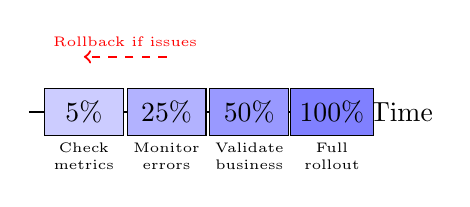
\begin{tikzpicture}[scale=0.7]
% Timeline
\draw[->, thick] (0,0) -- (6,0) node[right] {Time};

% Stages
\node[draw, fill=blue!20, minimum width=1cm, minimum height=0.6cm] at (1,0) {5\%};
\node[draw, fill=blue!30, minimum width=1cm, minimum height=0.6cm] at (2.5,0) {25\%};
\node[draw, fill=blue!40, minimum width=1cm, minimum height=0.6cm] at (4,0) {50\%};
\node[draw, fill=blue!50, minimum width=1cm, minimum height=0.6cm] at (5.5,0) {100\%};

% Checkpoints
\node[font=\tiny, align=center] at (1,-0.8) {Check\\metrics};
\node[font=\tiny, align=center] at (2.5,-0.8) {Monitor\\errors};
\node[font=\tiny, align=center] at (4,-0.8) {Validate\\business};
\node[font=\tiny, align=center] at (5.5,-0.8) {Full\\rollout};

% Rollback option
\draw[->, thick, red, dashed] (2.5,1) -- (1,1) node[midway, above, font=\tiny] {Rollback if issues};
\end{tikzpicture}

\vspace{0.5cm}
\textbf{Key Metrics to Monitor:}
\begin{itemize}
\item Prediction latency (p50, p99)
\item Error rates
\item Prediction distribution
\item Business KPIs (conversion, revenue)
\item Data drift indicators
\end{itemize}
\end{column}
\end{columns}
\end{frame}

% ============================================================================
% SECTION 2: DATA QUALITY AND MONITORING
% ============================================================================

\section{Data Quality and Monitoring}

\begin{frame}{The Hidden Technical Debt in ML Systems}
\begin{center}
\includegraphics[width=0.7\textwidth]{figures/ml_technical_debt.png}
\end{center}

\textbf{Key Insight from Google \cite{sculley2015hidden}:}
\begin{itemize}
\item ML code is only 5-10\% of production ML systems
\item 90-95\% is infrastructure: data, monitoring, configuration, serving
\item \textcolor{crimson}{\textbf{Data quality is the \#1 cause of model failures}}
\end{itemize}

\vspace{0.2cm}
\textbf{Costly Failures:}
\begin{itemize}
\item \textbf{Amazon (2018):} $50M revenue loss from recommendation system bug
\item \textbf{Knight Capital (2012):} $440M loss in 45 minutes from deployment error
\item \textbf{Target (2017):} Inventory system failure from data pipeline issues
\end{itemize}
\end{frame}

\begin{frame}{Data Quality Dimensions}
\begin{table}
\centering
\small
\begin{tabular}{p{2.5cm}p{4cm}p{4cm}}
\toprule
\textbf{Dimension} & \textbf{Definition} & \textbf{Detection Method} \\
\midrule
Completeness & No missing values & Null rate monitoring \\
\midrule
Consistency & Same meaning across sources & Schema validation \\
\midrule
Accuracy & Values match reality & Business rule checks \\
\midrule
Timeliness & Data arrives on schedule & Freshness monitoring \\
\midrule
Validity & Values within expected range & Distribution tests \\
\midrule
Uniqueness & No unexpected duplicates & Duplicate detection \\
\bottomrule
\end{tabular}
\end{table}

\vspace{0.3cm}
\textbf{Rule of Thumb:}
\begin{itemize}
\item Fix data quality issues \textcolor{crimson}{upstream} (in pipelines)
\item Don't try to fix bad data with better models
\item "Garbage in, garbage out" still applies to ML
\end{itemize}
\end{frame}

\begin{frame}[fragile]{Data Validation with Great Expectations}
\begin{lstlisting}[basicstyle=\ttfamily\tiny]
import great_expectations as ge

# Load data with expectations
df = ge.read_csv('transactions.csv')

# Define expectations (data quality rules)
df.expect_column_values_to_not_be_null('customer_id')
df.expect_column_values_to_be_unique('transaction_id')
df.expect_column_values_to_be_between('amount', min_value=0, max_value=10000)
df.expect_column_values_to_be_in_set('status', ['approved', 'declined', 'pending'])
df.expect_column_mean_to_be_between('amount', min_value=50, max_value=200)

# Custom expectation for business logic
df.expect_column_pair_values_to_be_equal(
    column_A='shipping_country',
    column_B='billing_country',
    mostly=0.95  # Allow 5% exceptions
)

# Validate and get report
validation_result = df.validate()
print(f"Success: {validation_result['success']}")
print(f"Statistics: {validation_result['statistics']}")

# Alert if validation fails
if not validation_result['success']:
    send_alert(f"Data quality check failed: {validation_result['results']}")
    raise ValueError("Data quality issues detected. Stopping pipeline.")
\end{lstlisting}

\textbf{Benefits:} Automated checks, versioned expectations, detailed reports
\end{frame}

\begin{frame}[fragile]{Data Drift Detection}
\textbf{Problem:} Production data distribution changes over time

\vspace{0.2cm}
\begin{lstlisting}[basicstyle=\ttfamily\tiny]
from scipy.stats import ks_2samp
from sklearn.metrics import pairwise_distances
import numpy as np

class DriftDetector:
    def __init__(self, reference_data, threshold=0.05):
        self.reference_data = reference_data
        self.threshold = threshold

    def detect_univariate_drift(self, new_data, feature):
        """Kolmogorov-Smirnov test for single feature"""
        reference_values = self.reference_data[feature].values
        new_values = new_data[feature].values

        statistic, p_value = ks_2samp(reference_values, new_values)

        drift_detected = p_value < self.threshold
        return {
            'feature': feature,
            'statistic': statistic,
            'p_value': p_value,
            'drift_detected': drift_detected
        }

    def detect_multivariate_drift(self, new_data, features):
        """Maximum Mean Discrepancy (MMD) for multivariate drift"""
        X_ref = self.reference_data[features].values
        X_new = new_data[features].values

        # Compute kernel matrices
        K_xx = pairwise_distances(X_ref, X_ref, metric='rbf')
        K_yy = pairwise_distances(X_new, X_new, metric='rbf')
        K_xy = pairwise_distances(X_ref, X_new, metric='rbf')

        # MMD statistic
        mmd = K_xx.mean() + K_yy.mean() - 2 * K_xy.mean()

        return {'mmd': mmd, 'drift_detected': mmd > 0.1}
\end{lstlisting}
\end{frame}

\begin{frame}[fragile]{Concept Drift Detection}
\textbf{Problem:} Relationship between features and target changes

\vspace{0.2cm}
\begin{lstlisting}[basicstyle=\ttfamily\tiny]
import numpy as np
from sklearn.metrics import accuracy_score

class ConceptDriftDetector:
    def __init__(self, window_size=1000, threshold=0.05):
        self.window_size = window_size
        self.threshold = threshold
        self.performance_history = []

    def update(self, y_true, y_pred):
        """Update with new batch of predictions and true labels"""
        accuracy = accuracy_score(y_true, y_pred)
        self.performance_history.append(accuracy)

        # Keep only recent history
        if len(self.performance_history) > 2 * self.window_size:
            self.performance_history = self.performance_history[-2*self.window_size:]

        # Detect drift if recent performance drops significantly
        if len(self.performance_history) >= 2 * self.window_size:
            recent_perf = np.mean(self.performance_history[-self.window_size:])
            baseline_perf = np.mean(self.performance_history[-2*self.window_size:-self.window_size])

            performance_drop = baseline_perf - recent_perf

            if performance_drop > self.threshold:
                return {
                    'drift_detected': True,
                    'baseline_performance': baseline_perf,
                    'current_performance': recent_perf,
                    'drop': performance_drop
                }

        return {'drift_detected': False}

# Usage in production
detector = ConceptDriftDetector(window_size=1000, threshold=0.05)

for batch in production_stream:
    predictions = model.predict(batch.X)

    # Wait for true labels (e.g., from user feedback)
    true_labels = get_true_labels(batch.ids, delay='1day')

    result = detector.update(true_labels, predictions)

    if result['drift_detected']:
        alert(f"Concept drift detected! Performance dropped by {result['drop']:.2%}")
        trigger_retraining_pipeline()
\end{lstlisting}
\end{frame}

\begin{frame}[fragile]{Model Performance Monitoring}
\textbf{Key Metrics to Track:}
\begin{columns}
\begin{column}{0.48\textwidth}
\textbf{Technical Metrics:}
\begin{itemize}
\item Accuracy, precision, recall
\item AUC-ROC, AUC-PR
\item Calibration error
\item Inference latency (p50, p95, p99)
\item Error rates and types
\item Resource utilization
\end{itemize}
\end{column}

\begin{column}{0.48\textwidth}
\textbf{Business Metrics:}
\begin{itemize}
\item Conversion rate impact
\item Revenue per prediction
\item Customer satisfaction
\item Operational costs
\item False positive/negative costs
\item Time to value
\end{itemize}
\end{column}
\end{columns}

\vspace{0.3cm}
\begin{lstlisting}[basicstyle=\ttfamily\tiny]
import prometheus_client as prom

# Define metrics
prediction_latency = prom.Histogram(
    'model_prediction_latency_seconds',
    'Time spent making prediction',
    buckets=[0.01, 0.05, 0.1, 0.5, 1.0]
)

prediction_counter = prom.Counter(
    'model_predictions_total',
    'Total number of predictions',
    ['model_version', 'prediction_class']
)

model_accuracy = prom.Gauge(
    'model_accuracy',
    'Current model accuracy',
    ['window']
)

# Instrument prediction endpoint
@prediction_latency.time()
def predict(features):
    prediction = model.predict(features)
    prediction_counter.labels(
        model_version='v1.2',
        prediction_class=str(prediction)
    ).inc()
    return prediction
\end{lstlisting}
\end{frame}

\begin{frame}{Monitoring Dashboard: Example Metrics}
\begin{center}
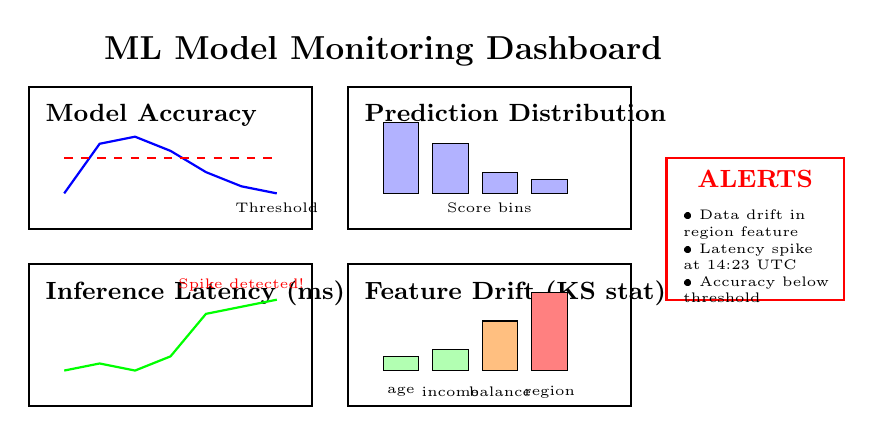
\begin{tikzpicture}[scale=0.9]
% Title
\node[font=\large\bfseries] at (5,5.5) {ML Model Monitoring Dashboard};

% 4 panels
% Panel 1: Accuracy over time
\draw[thick] (0,3) rectangle (4,5);
\node[anchor=north west, font=\small\bfseries] at (0.1,4.9) {Model Accuracy};
\draw[blue, thick] (0.5,3.5) -- (1,4.2) -- (1.5,4.3) -- (2,4.1) -- (2.5,3.8) -- (3,3.6) -- (3.5,3.5);
\draw[red, dashed] (0.5,4.0) -- (3.5,4.0);
\node[font=\tiny] at (3.5,3.3) {Threshold};

% Panel 2: Prediction distribution
\draw[thick] (4.5,3) rectangle (8.5,5);
\node[anchor=north west, font=\small\bfseries] at (4.6,4.9) {Prediction Distribution};
\draw[fill=blue!30] (5,3.5) rectangle (5.5,4.5);
\draw[fill=blue!30] (5.7,3.5) rectangle (6.2,4.2);
\draw[fill=blue!30] (6.4,3.5) rectangle (6.9,3.8);
\draw[fill=blue!30] (7.1,3.5) rectangle (7.6,3.7);
\node[font=\tiny] at (6.5,3.3) {Score bins};

% Panel 3: Latency
\draw[thick] (0,0.5) rectangle (4,2.5);
\node[anchor=north west, font=\small\bfseries] at (0.1,2.4) {Inference Latency (ms)};
\draw[green, thick] (0.5,1) -- (1,1.1) -- (1.5,1.0) -- (2,1.2) -- (2.5,1.8) -- (3,1.9) -- (3.5,2.0);
\node[font=\tiny, red] at (3,2.2) {Spike detected!};

% Panel 4: Data drift
\draw[thick] (4.5,0.5) rectangle (8.5,2.5);
\node[anchor=north west, font=\small\bfseries] at (4.6,2.4) {Feature Drift (KS stat)};
\draw[fill=green!30] (5,1) rectangle (5.5,1.2) node[midway, font=\tiny] {};
\draw[fill=green!30] (5.7,1) rectangle (6.2,1.3);
\draw[fill=orange!50] (6.4,1) rectangle (6.9,1.7);
\draw[fill=red!50] (7.1,1) rectangle (7.6,2.1);
\node[font=\tiny] at (5.25,0.7) {age};
\node[font=\tiny] at (5.95,0.7) {income};
\node[font=\tiny] at (6.65,0.7) {balance};
\node[font=\tiny] at (7.35,0.7) {region};

% Alert box
\draw[thick, red] (9,2) rectangle (11.5,4);
\node[font=\small\bfseries, red] at (10.25,3.7) {ALERTS};
\node[font=\tiny, align=left, anchor=north west] at (9.1,3.4) {
• Data drift in\\
  region feature\\
• Latency spike\\
  at 14:23 UTC\\
• Accuracy below\\
  threshold
};
\end{tikzpicture}
\end{center}

\vspace{0.2cm}
\small\textbf{Tools:} Grafana, Kibana, Datadog, Neptune.ai, Weights \& Biases
\end{frame}

\begin{frame}[fragile]{Alerting Strategy}
\textbf{Multi-Level Alert System:}
\begin{lstlisting}[basicstyle=\ttfamily\tiny]
class AlertingSystem:
    def __init__(self):
        self.alert_configs = {
            'CRITICAL': {
                'accuracy_drop': 0.10,      # 10% drop → page on-call
                'error_rate': 0.05,         # 5% errors → immediate action
                'latency_p99': 1000,        # 1s latency → scale up
                'channels': ['pagerduty', 'slack', 'email']
            },
            'WARNING': {
                'accuracy_drop': 0.05,      # 5% drop → investigate
                'data_drift_pvalue': 0.01,  # Significant drift
                'latency_p99': 500,         # 500ms latency
                'channels': ['slack', 'email']
            },
            'INFO': {
                'accuracy_drop': 0.02,      # 2% drop → monitor
                'prediction_volume': 0.20,  # 20% volume change
                'channels': ['email']
            }
        }

    def check_metrics(self, current_metrics, baseline_metrics):
        alerts = []

        # Check accuracy
        acc_drop = baseline_metrics['accuracy'] - current_metrics['accuracy']
        if acc_drop >= self.alert_configs['CRITICAL']['accuracy_drop']:
            alerts.append({
                'level': 'CRITICAL',
                'metric': 'accuracy',
                'message': f'Accuracy dropped by {acc_drop:.2%}',
                'action': 'Rollback to previous model version'
            })

        # Check latency
        if current_metrics['latency_p99'] > self.alert_configs['CRITICAL']['latency_p99']:
            alerts.append({
                'level': 'CRITICAL',
                'metric': 'latency',
                'message': f'P99 latency: {current_metrics["latency_p99"]}ms',
                'action': 'Scale up inference servers'
            })

        return alerts
\end{lstlisting}
\end{frame>

\begin{frame}{Model Retraining Strategies}
\textbf{When to Retrain:}
\begin{enumerate}
\item \textbf{Time-based (scheduled):} Daily, weekly, monthly
\item \textbf{Performance-based:} Accuracy drops below threshold
\item \textbf{Data-based:} Drift detected or new data volume threshold
\item \textbf{Event-based:} Business rule changes, new product launch
\end{enumerate}

\vspace{0.3cm}
\begin{columns}
\begin{column}{0.48\textwidth}
\textbf{Retraining Decision Matrix:}
\begin{table}
\tiny
\begin{tabular}{p{1.5cm}p{1.2cm}p{1.2cm}}
\toprule
\textbf{Model Type} & \textbf{Frequency} & \textbf{Trigger} \\
\midrule
Fraud detection & Daily & Performance \\
Recommendation & Weekly & Time + data \\
Credit scoring & Monthly & Regulatory \\
Churn prediction & Weekly & Data drift \\
\bottomrule
\end{tabular}
\end{table}
\end{column}

\begin{column}{0.48\textwidth}
\textbf{Retraining Pipeline:}
\begin{enumerate}
\item Detect trigger
\item Validate new data quality
\item Train candidate model
\item Run A/B test vs. current
\item Validate business metrics
\item Deploy if improved
\item Document changes
\end{enumerate}
\end{column}
\end{columns}

\vspace{0.3cm}
\textbf{Cost-Benefit Analysis:}
\begin{itemize}
\item Training compute cost vs. improved performance
\item Don't retrain if marginal improvement < threshold (e.g., 1\% accuracy gain)
\end{itemize}
\end{frame}

% ============================================================================
% SECTION 3: BUSINESS STAKEHOLDER COMMUNICATION
% ============================================================================

\section{Business Stakeholder Communication}

\begin{frame}{The Communication Challenge}
\begin{columns}
\begin{column}{0.55\textwidth}
\textbf{Why 87\% of ML Projects Fail:}
\begin{enumerate}
\item \textcolor{crimson}{Misaligned expectations} (35\%)
\item Lack of business value clarity (28\%)
\item Poor communication (24\%)
\item Technical issues (13\%)
\end{enumerate}

\vspace{0.3cm}
\textbf{Common Pitfalls:}
\begin{itemize}
\item Focusing on accuracy instead of business impact
\item Not quantifying expected ROI
\item Overpromising capabilities
\item Using technical jargon
\item Not involving stakeholders early
\end{itemize}
\end{column}

\begin{column}{0.4\textwidth}
\begin{center}
\textbf{Stakeholder Perspective}
\end{center}

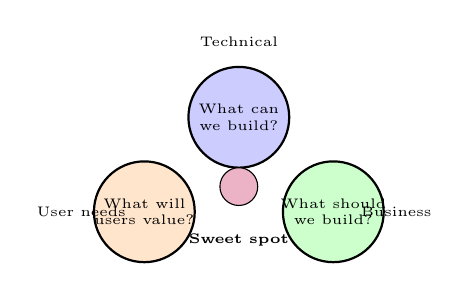
\begin{tikzpicture}[scale=0.8]
% Three circles
\draw[fill=blue!20, thick] (0,2) circle (0.8cm) node[font=\tiny, align=center] {What can\\we build?};
\draw[fill=green!20, thick] (1.5,0.5) circle (0.8cm) node[font=\tiny, align=center] {What should\\we build?};
\draw[fill=orange!20, thick] (-1.5,0.5) circle (0.8cm) node[font=\tiny, align=center] {What will\\users value?};

% Intersection
\draw[fill=purple!30] (0,0.9) circle (0.3cm);
\node[font=\tiny\bfseries, anchor=north] at (0,0.3) {Sweet spot};

% Labels
\node[font=\tiny] at (0,3.2) {Technical};
\node[font=\tiny] at (2.5,0.5) {Business};
\node[font=\tiny] at (-2.5,0.5) {User needs};
\end{tikzpicture}
\end{center}
\end{column}
\end{columns}

\vspace{0.3cm}
\textbf{Key Principle:} \textit{Translate technical achievements into business value}
\end{frame}

\begin{frame}{Speaking the Language of Business}
\textbf{Translation Guide:}
\begin{table}
\centering
\small
\begin{tabular}{p{4cm}p{6.5cm}}
\toprule
\textcolor{crimson}{\textbf{Don't Say (Technical)}} & \textcolor{forest}{\textbf{Do Say (Business)}} \\
\midrule
"Our AUC-ROC is 0.92" & "We correctly identify 92\% of high-risk customers, reducing review costs by \$2M/year" \\
\midrule
"We reduced loss from 0.45 to 0.32" & "Model predictions are 30\% more accurate, enabling better inventory decisions" \\
\midrule
"We implemented gradient boosting" & "We upgraded our algorithm, improving forecast accuracy from 75\% to 85\%" \\
\midrule
"Precision increased to 0.88" & "Of customers we target, 88\% convert—up from 65\%, doubling campaign ROI" \\
\midrule
"We need more GPU compute" & "To serve 10K predictions/sec (next quarter's traffic), we need \$5K/month infrastructure" \\
\bottomrule
\end{tabular}
\end{table}

\vspace{0.2cm}
\textbf{Framework:} [Metric] → [Business Impact] → [Financial Value]
\end{frame}

\begin{frame}[fragile]{Building a Business Case}
\textbf{Template: ML Project Proposal}

\begin{block}{1. Problem Statement (Business, not technical)}
\textit{Example:} "Customer churn costs us \$12M annually. We lose 15\% of customers each year, and acquiring replacements costs 5× retention."
\end{block}

\begin{block}{2. Proposed Solution}
\textit{Example:} "Build a churn prediction model to identify at-risk customers 30 days in advance, enabling proactive retention campaigns."
\end{block}

\begin{block}{3. Expected Business Value}
\begin{itemize}
\item \textbf{Primary KPI:} Reduce churn rate from 15\% to 11\% → \$3.2M annual savings
\item \textbf{Secondary KPIs:}
  \begin{itemize}
  \item Increase customer lifetime value by 8\%
  \item Improve retention campaign ROI from 120\% to 180\%
  \end{itemize}
\end{itemize}
\end{block}

\begin{block}{4. Investment Required}
\begin{itemize}
\item Data science team: 3 months × 2 FTE = \$120K
\item Infrastructure: \$15K (one-time) + \$3K/month ongoing
\item \textbf{Total first-year cost:} \$171K
\item \textbf{Expected ROI:} 18.7× (\$3.2M / \$171K)
\item \textbf{Payback period:} 21 days
\end{itemize}
\end{block}
\end{frame}

\begin{frame}{Quantifying Model Value: Example Calculations}
\textbf{Confusion Matrix → Business Impact}

\begin{columns}
\begin{column}{0.48\textwidth}
\textbf{Fraud Detection Model:}
\begin{table}
\tiny
\begin{tabular}{lcc}
\toprule
& \textbf{Actual Fraud} & \textbf{Actual Legit} \\
\midrule
\textbf{Predicted Fraud} & 950 (TP) & 200 (FP) \\
\textbf{Predicted Legit} & 50 (FN) & 9800 (TN) \\
\bottomrule
\end{tabular}
\end{table}

\textbf{Business Costs:}
\begin{itemize}
\item TP: \$0 (fraud caught)
\item TN: \$0 (correct)
\item FP: \$25 (manual review)
\item FN: \$500 (fraud missed)
\end{itemize}

\textbf{Total Cost:}
\begin{align*}
\text{Cost} &= 200 \times \$25 + 50 \times \$500 \\
&= \$5,000 + \$25,000 = \$30,000
\end{align*}

\textbf{Without Model:}
\begin{align*}
\text{Cost} &= 1,000 \times \$500 = \$500,000
\end{align*}

\textcolor{forest}{\textbf{Value: \$470K saved per 10K transactions}}
\end{column}

\begin{column}{0.48\textwidth}
\textbf{Marketing Campaign Model:}
\begin{table}
\tiny
\begin{tabular}{lcc}
\toprule
& \textbf{Will Convert} & \textbf{Won't Convert} \\
\midrule
\textbf{Targeted} & 1,800 (TP) & 200 (FP) \\
\textbf{Not Targeted} & 200 (FN) & 7,800 (TN) \\
\bottomrule
\end{tabular}
\end{table}

\textbf{Business Economics:}
\begin{itemize}
\item Campaign cost: \$10 per customer
\item Conversion value: \$100
\end{itemize}

\textbf{With Model (targeting 2,000):}
\begin{align*}
\text{Revenue} &= 1,800 \times \$100 = \$180,000 \\
\text{Cost} &= 2,000 \times \$10 = \$20,000 \\
\text{Profit} &= \$160,000 \\
\text{ROI} &= 800\%
\end{align*}

\textbf{Without Model (mass mailing 10,000):}
\begin{align*}
\text{Revenue} &= 2,000 \times \$100 = \$200,000 \\
\text{Cost} &= 10,000 \times \$10 = \$100,000 \\
\text{Profit} &= \$100,000 \\
\text{ROI} &= 100\%
\end{align*}

\textcolor{forest}{\textbf{Value: \$60K additional profit}}
\end{column}
\end{columns}
\end{frame}

\begin{frame}{Presenting Model Performance to Executives}
\textbf{Good Visualization Example:}

\begin{center}
\begin{tikzpicture}[scale=0.9]
% Title
\node[font=\large\bfseries] at (5,5.5) {Churn Prediction Model: Business Impact};

% Left panel: Bar chart of savings
\node[anchor=north west, font=\small\bfseries] at (0,5) {Annual Cost Savings};
\draw[fill=red!30] (0.5,2.5) rectangle (2,4.5) node[midway, rotate=90] {\$12M};
\draw[fill=green!50] (2.5,2.5) rectangle (4,1.5) node[midway, rotate=90] {\$8.8M};
\node[font=\small] at (1.25,2.2) {Without Model};
\node[font=\small] at (3.25,2.2) {With Model};
\draw[<->, thick] (4.5,1.5) -- (4.5,4.5) node[midway, right, font=\small] {\textcolor{forest}{\$3.2M saved}};

% Right panel: Accuracy breakdown
\node[anchor=north west, font=\small\bfseries] at (6,5) {Model Accuracy};
\node[font=\small, align=left, anchor=north west] at (6,4.5) {
\textcolor{forest}{✓} 78\% of churners identified\\
\textcolor{green}{✓} 92\% of loyal customers correct\\
\textcolor{orange}{⚠} 22\% churners missed\\
\textcolor{blue}{ℹ} 8\% false alarms
};

% Bottom: Timeline
\node[anchor=north west, font=\small\bfseries] at (0,1.5) {Rollout Plan};
\draw[->, thick] (0.5,0.2) -- (10,0.2);
\node[draw, fill=blue!20, font=\tiny] at (2,0.2) {Q1: Pilot};
\node[draw, fill=blue!30, font=\tiny] at (4.5,0.2) {Q2: 50\% scale};
\node[draw, fill=blue!40, font=\tiny] at (7,0.2) {Q3: Full rollout};
\node[draw, fill=green!40, font=\tiny] at (9.5,0.2) {Q4: \$3.2M saved};
\end{tikzpicture}
\end{center}

\textbf{Key Principles:}
\begin{itemize}
\item Lead with business metrics (\$), not technical metrics (AUC)
\item Use comparisons ("With vs. Without Model")
\item Include confidence levels and risks
\item Show clear timeline and milestones
\end{itemize}
\end{frame>

\begin{frame}{Managing Expectations: ML Limitations}
\textbf{Be Transparent About:}

\begin{columns}
\begin{column}{0.48\textwidth}
\textbf{What ML Can Do:}
\begin{itemize}
\item Find patterns in historical data
\item Automate repetitive decisions
\item Handle complexity beyond rules
\item Improve with more data
\item Provide probabilistic predictions
\end{itemize}
\end{column}

\begin{column}{0.48\textwidth}
\textbf{What ML Cannot Do:}
\begin{itemize}
\item Predict unprecedented events
\item Explain causality automatically
\item Work without quality data
\item Eliminate all errors
\item Replace domain expertise
\end{itemize}
\end{column}
\end{columns}

\vspace{0.4cm}
\textbf{Common Misconceptions to Address:}

\begin{enumerate}
\item \textcolor{crimson}{\textbf{"AI will be 100\% accurate"}}
  \begin{itemize}
  \item \textit{Reality:} All models make errors. Focus on cost-benefit analysis.
  \end{itemize}

\item \textcolor{crimson}{\textbf{"Once deployed, it will work forever"}}
  \begin{itemize}
  \item \textit{Reality:} Models degrade. Requires monitoring and retraining.
  \end{itemize}

\item \textcolor{crimson}{\textbf{"More data always helps"}}
  \begin{itemize}
  \item \textit{Reality:} Data quality > quantity. Bad data → bad models.
  \end{itemize}

\item \textcolor{crimson}{\textbf{"The model will explain why"}}
  \begin{itemize}
  \item \textit{Reality:} Correlation ≠ causation. Model shows "what," not "why."
  \end{itemize}
\end{enumerate}
\end{frame}

\begin{frame}{Stakeholder Communication Framework}
\textbf{Tailored Communication by Role:}

\begin{table}
\centering
\small
\begin{tabular}{p{2cm}p{3.5cm}p{5cm}}
\toprule
\textbf{Stakeholder} & \textbf{Primary Concern} & \textbf{Key Message} \\
\midrule
\textbf{Executives} & ROI, risk, timeline & "\$X value in Y months with Z\% confidence" \\
\midrule
\textbf{Product} & Features, user impact & "Users see A, which enables B, measured by C" \\
\midrule
\textbf{Engineering} & Integration, scalability & "API design, latency SLAs, infrastructure needs" \\
\midrule
\textbf{Legal/Compliance} & Regulations, risk & "GDPR compliance, audit trails, bias testing" \\
\midrule
\textbf{Domain Experts} & Accuracy, edge cases & "Model handles X well, struggles with Y, needs review for Z" \\
\bottomrule
\end{tabular}
\end{table}

\vspace{0.3cm}
\textbf{Communication Cadence:}
\begin{itemize}
\item \textbf{Development:} Bi-weekly demos, monthly business reviews
\item \textbf{Pre-launch:} Risk assessment, integration test results
\item \textbf{Post-launch:} Weekly monitoring reports, monthly business impact
\item \textbf{Ad-hoc:} Immediate alerts for critical issues
\end{itemize}
\end{frame}

\begin{frame}[fragile]{Model Documentation for Non-Technical Stakeholders}
\textbf{Model Card Template:}

\begin{block}{Executive Summary (1 paragraph)}
"This model predicts customer churn 30 days in advance with 78\% accuracy. Deployed in Q2 2024, it has reduced churn from 15\% to 11\%, saving \$3.2M annually. The model is retrained monthly and monitored daily for performance degradation."
\end{block}

\begin{block}{Business Context}
\begin{itemize}
\item \textbf{Problem:} High customer churn costing \$12M/year
\item \textbf{Solution:} Proactive retention campaigns for at-risk customers
\item \textbf{Impact:} 26\% reduction in churn rate
\item \textbf{Users:} Customer success team (15 people)
\end{itemize}
\end{block}

\begin{block}{Model Performance (in plain language)}
\begin{itemize}
\item \textbf{Accuracy:} Correctly predicts churn in 78 out of 100 cases
\item \textbf{False Alarms:} 8\% of customers flagged don't actually churn (acceptable cost)
\item \textbf{Missed Cases:} 22\% of churners not detected (acceptable given ROI)
\item \textbf{Confidence:} High for customers with 6+ months history, medium for new customers
\end{itemize}
\end{block}

\begin{block}{Limitations and Risks}
\begin{itemize}
\item Cannot predict churn caused by external shocks (e.g., competitor launches)
\item Performance degrades without monthly retraining
\item Requires 6 months historical data per customer
\end{itemize}
\end{block}
\end{frame}

% ============================================================================
% SECTION 4: REGULATORY COMPLIANCE AND ETHICS
% ============================================================================

\section{Regulatory Compliance and Ethics}

\begin{frame}{The Regulatory Landscape}
\textbf{Major ML Regulations (2024):}

\begin{table}
\centering
\small
\begin{tabular}{p{2.5cm}p{3cm}p{5cm}}
\toprule
\textbf{Regulation} & \textbf{Region} & \textbf{Key Requirements} \\
\midrule
\textbf{EU AI Act} & European Union & Risk classification, transparency, human oversight, prohibited uses \\
\midrule
\textbf{GDPR} & EU/EEA & Right to explanation, data minimization, consent \\
\midrule
\textbf{CCPA/CPRA} & California & Consumer data rights, automated decision-making disclosure \\
\midrule
\textbf{FCRA} & USA (Finance) & Fair credit reporting, adverse action notices \\
\midrule
\textbf{ECOA} & USA (Lending) & Prohibition of discriminatory lending practices \\
\midrule
\textbf{HIPAA} & USA (Healthcare) & Protected health information, data security \\
\bottomrule
\end{tabular}
\end{table}

\vspace{0.3cm}
\textbf{Penalties for Non-Compliance:}
\begin{itemize}
\item \textbf{GDPR:} Up to €20M or 4\% of global revenue (whichever is higher)
\item \textbf{EU AI Act:} Up to €35M or 7\% of global revenue for high-risk violations
\item \textbf{CCPA:} Up to \$7,500 per violation
\end{itemize}
\end{frame}

\begin{frame}{EU AI Act: Risk-Based Approach}
\begin{table}
\centering
\small
\begin{tabular}{p{2.2cm}p{3.5cm}p{4.8cm}}
\toprule
\textbf{Risk Level} & \textbf{Examples} & \textbf{Requirements} \\
\midrule
\textcolor{crimson}{\textbf{Unacceptable}} & Social scoring, emotion recognition in schools & \textbf{Prohibited} \\
\midrule
\textcolor{orange}{\textbf{High-Risk}} & Credit scoring, hiring, healthcare diagnosis, law enforcement & • Conformity assessment\\
• Transparency\\
• Human oversight\\
• Robustness testing\\
• Audit trail \\
\midrule
\textcolor{gold}{\textbf{Limited Risk}} & Chatbots, deepfakes & • Transparency obligations\\
• User disclosure \\
\midrule
\textcolor{forest}{\textbf{Minimal Risk}} & Spam filters, video games & • No obligations \\
\bottomrule
\end{tabular}
\end{table}

\vspace{0.2cm}
\textbf{Key Compliance Requirements for High-Risk AI:}
\begin{itemize}
\item Risk management system
\item Data governance and quality
\item Technical documentation (model cards)
\item Record-keeping (logging predictions)
\item Transparency and user information
\item Human oversight mechanisms
\item Accuracy, robustness, cybersecurity
\end{itemize}
\end{frame}

\begin{frame}{GDPR: Right to Explanation}
\textbf{Article 22: Automated Decision-Making}

\textit{"The data subject shall have the right not to be subject to a decision based solely on automated processing, including profiling, which produces legal effects..."}

\vspace{0.3cm}
\textbf{Practical Implications:}
\begin{enumerate}
\item \textbf{Right to meaningful information:} Users must understand how decisions are made
\item \textbf{Right to human intervention:} Option to contest automated decisions
\item \textbf{Right to explanation:} Understand logic behind decisions (debated scope)
\end{enumerate}

\vspace{0.3cm}
\textbf{Compliance Strategies:}
\begin{itemize}
\item Use interpretable models when possible (decision trees, linear models)
\item Provide feature importance for black-box models
\item Implement LIME/SHAP for individual explanations
\item Document model development and validation
\item Establish human review processes for contested decisions
\item Maintain audit logs of all automated decisions
\end{itemize}

\vspace{0.2cm}
\textit{Note: "Right to explanation" interpretation varies by jurisdiction and is subject to ongoing legal clarification}
\end{frame>

\begin{frame}[fragile]{Implementing Explainability for Compliance}
\textbf{Example: LIME for Individual Predictions}
\begin{lstlisting}[basicstyle=\ttfamily\tiny]
import lime
import lime.lime_tabular
from sklearn.ensemble import RandomForestClassifier

# Train model
model = RandomForestClassifier(n_estimators=100)
model.fit(X_train, y_train)

# Create LIME explainer
explainer = lime.lime_tabular.LimeTabularExplainer(
    X_train.values,
    feature_names=feature_names,
    class_names=['Approved', 'Denied'],
    mode='classification'
)

# Explain a specific prediction (e.g., loan application)
instance = X_test.iloc[42]  # Application that was denied
explanation = explainer.explain_instance(
    instance.values,
    model.predict_proba,
    num_features=10
)

# Generate human-readable explanation
print("Prediction: Denied")
print("\nTop factors contributing to this decision:")
for feature, weight in explanation.as_list():
    if weight < 0:  # Negative weight = contributes to denial
        print(f"  • {feature}: {weight:.3f}")

# Example output:
# Top factors contributing to this decision:
#   • Income < 50000: -0.23
#   • Credit_Score < 650: -0.19
#   • Debt_to_Income_Ratio > 0.45: -0.15

# Save explanation for audit trail
explanation.save_to_file(f'explanations/application_{applicant_id}.html')
\end{lstlisting}

\textbf{For adverse action notices (required by FCRA):}
\begin{itemize}
\item Primary factors must be specific, understandable, and actionable
\item Example: "Credit score below threshold (650)" not "Feature X = 0.23"
\end{itemize}
\end{frame}

\begin{frame}[fragile]{Model Auditing and Documentation}
\textbf{Audit Trail Requirements:}
\begin{lstlisting}[basicstyle=\ttfamily\tiny]
import json
import hashlib
from datetime import datetime

class ModelAuditLogger:
    def __init__(self, model_name, version):
        self.model_name = model_name
        self.version = version

    def log_prediction(self, input_data, prediction, user_id=None):
        """Log every prediction for compliance"""
        audit_record = {
            'timestamp': datetime.utcnow().isoformat(),
            'model_name': self.model_name,
            'model_version': self.version,
            'user_id': user_id,
            'input_hash': hashlib.sha256(
                json.dumps(input_data, sort_keys=True).encode()
            ).hexdigest(),  # Hash PII for privacy
            'prediction': prediction,
            'explanation': self.generate_explanation(input_data, prediction)
        }

        # Write to append-only log (for auditability)
        with open(f'audit_logs/{self.model_name}_{datetime.now():%Y%m%d}.jsonl', 'a') as f:
            f.write(json.dumps(audit_record) + '\n')

        return audit_record

    def generate_explanation(self, input_data, prediction):
        """Generate human-readable explanation"""
        # Use SHAP or LIME
        explanation = self.explainer.explain(input_data)
        return {
            'top_features': explanation.top_k(5),
            'confidence': prediction['probability'],
            'model_uncertainty': self.estimate_uncertainty(input_data)
        }

# Usage in production
logger = ModelAuditLogger(model_name='credit_scoring', version='v2.1')

prediction = model.predict_proba(applicant_data)
audit_record = logger.log_prediction(
    input_data=applicant_data,
    prediction={'class': 'denied', 'probability': 0.73},
    user_id=applicant_id
)
\end{lstlisting}

\textbf{Retention:} GDPR requires logs for contested decisions. FCRA requires 2 years for credit.
\end{frame}

\begin{frame}{Bias Detection and Mitigation}
\textbf{Legal Requirements:}
\begin{itemize}
\item \textbf{Equal Credit Opportunity Act (ECOA):} Prohibits discrimination by race, color, religion, national origin, sex, marital status, age
\item \textbf{Fair Housing Act:} Prohibits discrimination in housing-related lending
\item \textbf{EU AI Act:} Requires bias testing for high-risk AI systems
\end{itemize}

\vspace{0.3cm}
\textbf{Protected Attributes (US):}
\begin{itemize}
\item Race, color, national origin
\item Sex, gender identity
\item Religion
\item Disability
\item Age (40+)
\item Marital status, familial status
\end{itemize}

\vspace{0.3cm}
\textbf{Types of Discrimination:}
\begin{enumerate}
\item \textcolor{crimson}{\textbf{Disparate Treatment:}} Explicit use of protected attributes (illegal)
\item \textcolor{orange}{\textbf{Disparate Impact:}} Facially neutral policy with discriminatory effect (requires justification)
\end{enumerate}

\textit{Example:} Using ZIP code as a feature may proxy for race, leading to disparate impact.
\end{frame}

\begin{frame}[fragile]{Fairness Testing for Compliance}
\begin{lstlisting}[basicstyle=\ttfamily\tiny]
from aif360.datasets import BinaryLabelDataset
from aif360.metrics import BinaryLabelDatasetMetric, ClassificationMetric

# Load data with protected attributes
dataset = BinaryLabelDataset(
    df=data,
    label_names=['approved'],
    protected_attribute_names=['race', 'sex']
)

# Test for disparate impact
metric = BinaryLabelDatasetMetric(
    dataset,
    unprivileged_groups=[{'race': 0}],  # Minority group
    privileged_groups=[{'race': 1}]     # Majority group
)

# 80% rule (EEOC guideline)
disparate_impact = metric.disparate_impact()
print(f"Disparate Impact Ratio: {disparate_impact:.3f}")

# Ratio < 0.8 suggests potential discrimination
if disparate_impact < 0.8:
    print("⚠️  Warning: Model may have disparate impact")
    print("   Consider: re-weighting, threshold adjustment, or fairness constraints")

# After model predictions
predictions = model.predict(X_test)
classified_metric = ClassificationMetric(
    dataset_test,
    predicted_dataset,
    unprivileged_groups=[{'race': 0}],
    privileged_groups=[{'race': 1}]
)

# Multiple fairness metrics
print(f"Equal Opportunity Difference: {classified_metric.equal_opportunity_difference():.3f}")
print(f"Average Odds Difference: {classified_metric.average_odds_difference():.3f}")
print(f"Predictive Parity Difference: {classified_metric.statistical_parity_difference():.3f}")

# Generate fairness report for compliance documentation
fairness_report = {
    'disparate_impact': disparate_impact,
    'statistical_parity_difference': classified_metric.statistical_parity_difference(),
    'equal_opportunity_difference': classified_metric.equal_opportunity_difference(),
    'pass_80_percent_rule': disparate_impact >= 0.8
}

with open('compliance/fairness_report.json', 'w') as f:
    json.dump(fairness_report, f, indent=2)
\end{lstlisting}
\end{frame>

\begin{frame}[fragile]{Bias Mitigation Techniques}
\textbf{Three-Stage Approach:}

\begin{columns}
\begin{column}{0.48\textwidth}
\textbf{1. Pre-processing (Data):}
\begin{lstlisting}[basicstyle=\ttfamily\tiny]
from aif360.algorithms.preprocessing import Reweighing

# Reweight training instances
rw = Reweighing(
    unprivileged_groups=[{'sex': 0}],
    privileged_groups=[{'sex': 1}]
)
dataset_transformed = rw.fit_transform(dataset)

# Train on reweighted data
model.fit(
    dataset_transformed.features,
    dataset_transformed.labels,
    sample_weight=dataset_transformed.instance_weights
)
\end{lstlisting}

\textbf{2. In-processing (Algorithm):}
\begin{lstlisting}[basicstyle=\ttfamily\tiny]
from aif360.algorithms.inprocessing import PrejudiceRemover

# Train with fairness constraint
model = PrejudiceRemover(
    sensitive_attr='sex',
    eta=1.0  # Fairness weight
)
model.fit(dataset)
\end{lstlisting}
\end{column}

\begin{column}{0.48\textwidth}
\textbf{3. Post-processing (Predictions):}
\begin{lstlisting}[basicstyle=\ttfamily\tiny]
from aif360.algorithms.postprocessing import EqOddsPostprocessing

# Adjust predictions for fairness
eop = EqOddsPostprocessing(
    unprivileged_groups=[{'sex': 0}],
    privileged_groups=[{'sex': 1}]
)
dataset_transf_pred = eop.fit_predict(
    dataset_val,
    dataset_pred
)
\end{lstlisting}

\vspace{0.2cm}
\textbf{Trade-offs:}
\begin{itemize}
\item Fairness ↔ Accuracy
\item Different fairness definitions conflict
\item May reduce overall performance
\end{itemize}

\textbf{Business Decision:}
\begin{itemize}
\item What accuracy drop is acceptable for fairness compliance?
\item Which fairness metric matches legal requirement?
\end{itemize}
\end{column}
\end{columns}
\end{frame>

\begin{frame}{Privacy-Preserving ML}
\textbf{Techniques for GDPR/CCPA Compliance:}

\begin{enumerate}
\item \textbf{Differential Privacy:}
\begin{itemize}
\item Add calibrated noise to data/models
\item Guarantees: Individual records don't significantly affect model
\item Example: Train with DP-SGD (differentially private stochastic gradient descent)
\item Privacy budget: $\varepsilon$ = 1.0 (strong), $\varepsilon$ = 10.0 (weak)
\end{itemize}

\item \textbf{Federated Learning:}
\begin{itemize}
\item Train on decentralized data without central collection
\item Each client trains locally, shares only model updates
\item Reduces data exposure risk
\end{itemize}

\item \textbf{Anonymization/Pseudonymization:}
\begin{itemize}
\item Remove direct identifiers before model training
\item K-anonymity: Each record indistinguishable from k-1 others
\item L-diversity: Sensitive attributes have diverse values
\end{itemize}

\item \textbf{Data Minimization:}
\begin{itemize}
\item Collect only necessary features
\item Retain data only as long as needed
\item Use aggregated features when possible
\end{itemize}
\end{enumerate}

\vspace{0.2cm}
\textbf{Right to be Forgotten:}
\begin{itemize}
\item Implement mechanisms to remove user data from training sets
\item May require model retraining
\item Consider machine unlearning techniques
\end{itemize}
\end{frame}

\begin{frame}[fragile]{Implementing Differential Privacy}
\begin{lstlisting}[basicstyle=\ttfamily\tiny]
from tensorflow_privacy.privacy.optimizers import dp_optimizer
import tensorflow as tf

# Standard training (not private)
optimizer = tf.keras.optimizers.SGD(learning_rate=0.01)

# Differentially private training
optimizer = dp_optimizer.DPKerasSGDOptimizer(
    l2_norm_clip=1.0,           # Gradient clipping threshold
    noise_multiplier=0.5,        # Noise scale
    num_microbatches=1,          # Microbatch size
    learning_rate=0.01
)

model.compile(optimizer=optimizer, loss='binary_crossentropy', metrics=['accuracy'])

# Compute privacy budget after training
from tensorflow_privacy.privacy.analysis import compute_dp_sgd_privacy

eps = compute_dp_sgd_privacy.compute_dp_sgd_privacy(
    n=len(X_train),              # Dataset size
    batch_size=250,
    noise_multiplier=0.5,
    epochs=10,
    delta=1e-5                   # Failure probability
)

print(f"Privacy guarantee: (ε={eps[0]:.2f}, δ={eps[1]})")
# Example output: Privacy guarantee: (ε=2.5, δ=1e-05)
# Interpretation: Privacy loss is bounded by ε=2.5

# Document privacy parameters for compliance
privacy_report = {
    'mechanism': 'DP-SGD',
    'epsilon': eps[0],
    'delta': eps[1],
    'noise_multiplier': 0.5,
    'l2_norm_clip': 1.0,
    'training_samples': len(X_train)
}
\end{lstlisting}

\textbf{Trade-off:} Lower $\varepsilon$ (stronger privacy) → Lower model accuracy
\end{frame}

\begin{frame}{Model Governance Framework}
\textbf{Organizational Structure:}

\begin{center}
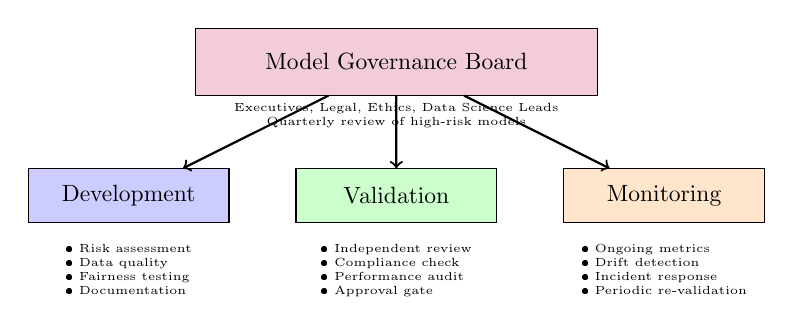
\begin{tikzpicture}[scale=0.85, every node/.style={scale=0.85}]
% Governance Board
\node[draw, rectangle, fill=purple!20, minimum width=6cm, minimum height=1cm] (board) at (5,4) {Model Governance Board};
\node[font=\tiny, align=center, anchor=north] at (5,3.5) {Executives, Legal, Ethics, Data Science Leads\\
Quarterly review of high-risk models};

% Three pillars
\node[draw, rectangle, fill=blue!20, minimum width=3cm, minimum height=0.8cm] (dev) at (1,2) {Development};
\node[draw, rectangle, fill=green!20, minimum width=3cm, minimum height=0.8cm] (val) at (5,2) {Validation};
\node[draw, rectangle, fill=orange!20, minimum width=3cm, minimum height=0.8cm] (mon) at (9,2) {Monitoring};

% Connections
\draw[->, thick] (board) -- (dev);
\draw[->, thick] (board) -- (val);
\draw[->, thick] (board) -- (mon);

% Details
\node[font=\tiny, align=left, anchor=north] at (1,1.4) {
• Risk assessment\\
• Data quality\\
• Fairness testing\\
• Documentation
};

\node[font=\tiny, align=left, anchor=north] at (5,1.4) {
• Independent review\\
• Compliance check\\
• Performance audit\\
• Approval gate
};

\node[font=\tiny, align=left, anchor=north] at (9,1.4) {
• Ongoing metrics\\
• Drift detection\\
• Incident response\\
• Periodic re-validation
};
\end{tikzpicture}
\end{center}

\vspace{0.2cm}
\textbf{Model Risk Tiers:}
\begin{itemize}
\item \textbf{Tier 1 (High):} Credit decisions, hiring, healthcare → Full board review, external audit
\item \textbf{Tier 2 (Medium):} Marketing, pricing → Internal review, documented approval
\item \textbf{Tier 3 (Low):} Recommendations, search → Standard processes, monitoring
\end{itemize}

\textbf{Approval Gates:}
\begin{enumerate}
\item Development complete → Validation review
\item Validation passed → Compliance approval
\item Compliance cleared → Production deployment
\item Quarterly → Re-validation for high-risk models
\end{enumerate}
\end{frame>

\begin{frame}{Ethical Considerations Beyond Compliance}
\textbf{Responsible AI Principles:}

\begin{columns}
\begin{column}{0.48\textwidth}
\textbf{1. Beneficence:} Do good
\begin{itemize}
\item Maximize societal benefit
\item Consider positive and negative impacts
\item Ensure accessibility
\end{itemize}

\vspace{0.2cm}
\textbf{2. Non-maleficence:} Do no harm
\begin{itemize}
\item Prevent misuse
\item Protect vulnerable populations
\item Safety by design
\end{itemize}

\vspace{0.2cm}
\textbf{3. Autonomy:} Preserve human agency
\begin{itemize}
\item Human oversight for critical decisions
\item Meaningful control
\item Contestability
\end{itemize}
\end{column}

\begin{column}{0.48\textwidth}
\textbf{4. Justice:} Promote fairness
\begin{itemize}
\item Equitable access
\item Fair outcomes across groups
\item Address historical biases
\end{itemize}

\vspace{0.2cm}
\textbf{5. Explicability:} Enable understanding
\begin{itemize}
\item Transparency
\item Interpretability
\item Clear communication
\end{itemize}
\end{column}
\end{columns}

\vspace{0.3cm}
\textbf{Ethical Red Flags:}
\begin{itemize}
\item Using data collected without informed consent
\item Optimizing for engagement without considering harms (e.g., addiction)
\item Deploying in high-stakes domains without human oversight
\item Ignoring fairness because "it's legal"
\item Not disclosing limitations to users
\end{itemize}

\vspace{0.2cm}
\textit{Remember: Compliance is the floor, not the ceiling. Ethical AI requires going beyond legal requirements.}
\end{frame}

\begin{frame}{Case Study: COMPAS Recidivism Algorithm}
\textbf{Background:}
\begin{itemize}
\item Correctional Offender Management Profiling for Alternative Sanctions (COMPAS)
\item Used by courts to assess recidivism risk in sentencing decisions
\item Proprietary algorithm (black box)
\end{itemize}

\vspace{0.2cm}
\textbf{ProPublica Investigation (2016) Found:}
\begin{itemize}
\item \textcolor{crimson}{Black defendants:} 45\% false positive rate (incorrectly labeled high risk)
\item \textcolor{forest}{White defendants:} 23\% false positive rate
\item Overall accuracy similar (~60\%) but error distribution biased
\item Race not explicitly used, but correlated features (ZIP code, employment) proxy for race
\end{itemize}

\vspace{0.2cm}
\textbf{Company Response:}
\begin{itemize}
\item Algorithm satisfies predictive parity (calibration)
\item Same score means same risk regardless of race
\item But: Different groups have different error rates (violates equalized odds)
\end{itemize}

\vspace{0.2cm}
\textbf{Lessons:}
\begin{enumerate}
\item Black-box models in high-stakes decisions → accountability problems
\item Competing fairness definitions → need stakeholder input on priorities
\item Technical fairness metrics ≠ societal fairness perceptions
\item Transparency and contestability are critical for trust
\end{enumerate}
\end{frame}

\begin{frame}{Practical Checklist: Industry-Ready ML}
\textbf{Before Deployment:}

\begin{columns}
\begin{column}{0.48\textwidth}
\textbf{MLOps:}
\begin{itemize}
\item[$\square$] Version control (code, data, models)
\item[$\square$] Reproducible training pipeline
\item[$\square$] Automated testing (unit, integration)
\item[$\square$] CI/CD pipeline
\item[$\square$] Containerization (Docker)
\item[$\square$] Monitoring and alerting setup
\item[$\square$] Rollback procedure documented
\end{itemize}

\vspace{0.2cm}
\textbf{Data Quality:}
\begin{itemize}
\item[$\square$] Data validation rules defined
\item[$\square$] Drift detection implemented
\item[$\square$] Feature store (if applicable)
\item[$\square$] Training-serving consistency check
\end{itemize}
\end{column}

\begin{column}{0.48\textwidth}
\textbf{Compliance:}
\begin{itemize}
\item[$\square$] Risk assessment completed
\item[$\square$] Fairness testing (if applicable)
\item[$\square$] Explainability mechanism
\item[$\square$] Audit logging implemented
\item[$\square$] Privacy review (PII handling)
\item[$\square$] Model card/documentation
\item[$\square$] Legal/compliance sign-off
\end{itemize}

\vspace{0.2cm}
\textbf{Business:}
\begin{itemize}
\item[$\square$] ROI quantified
\item[$\square$] Success metrics defined
\item[$\square$] Stakeholder training completed
\item[$\square$] Incident response plan
\item[$\square$] Business continuity (if model fails)
\end{itemize}
\end{column}
\end{columns}

\vspace{0.3cm}
\textbf{Post-Deployment:}
\begin{itemize}
\item[$\square$] Weekly monitoring reports
\item[$\square$] Monthly business impact review
\item[$\square$] Quarterly re-validation (high-risk models)
\item[$\square$] Continuous improvement based on feedback
\end{itemize}
\end{frame}

% ============================================================================
% END OF INDUSTRY FOCUS ENHANCEMENTS
% ============================================================================
